\chapter{Fashion Recommendation}
\label{chapter-fashion-recommendation}
\begin{ChapAbstract}
In this chapter, we address the problem of recommending items given a reference fashion item. We carefully investigate three approaches to retrieving items: similar items within the same category, complementary items from other categories, and items guided by text feedback. 
In terms of retrieving intra-category similar items and text feedback-guided items, we employ a pretrained CLIP-based model and receive remarkable results. As for the inter-category complementary item retrieval, we consider it a Natural Language Process problem and propose Outfit Retrieval Transformers (ORT), which utilizes the Transformers architecture. Through experiments, ORT proves its effectiveness and can produce reasonable recommendations. Because using an embedding to query items from a dataset plays an important role in recommendation, we analyze various approximate searching methods and compare them with the exhaustive K-Nearest Neighbor algorithm regarding query time and accuracy.
\end{ChapAbstract}

\section{Overview}
Fashion recommendation involves retrieving items from a fashion dataset based on some given information and proposing them to users. To limit the scope, in this thesis, we take an input garment as the reference item and investigate three approaches to retrieving items based on the visual feature of that item. 

\begin{figure}[t!]
    \centering
    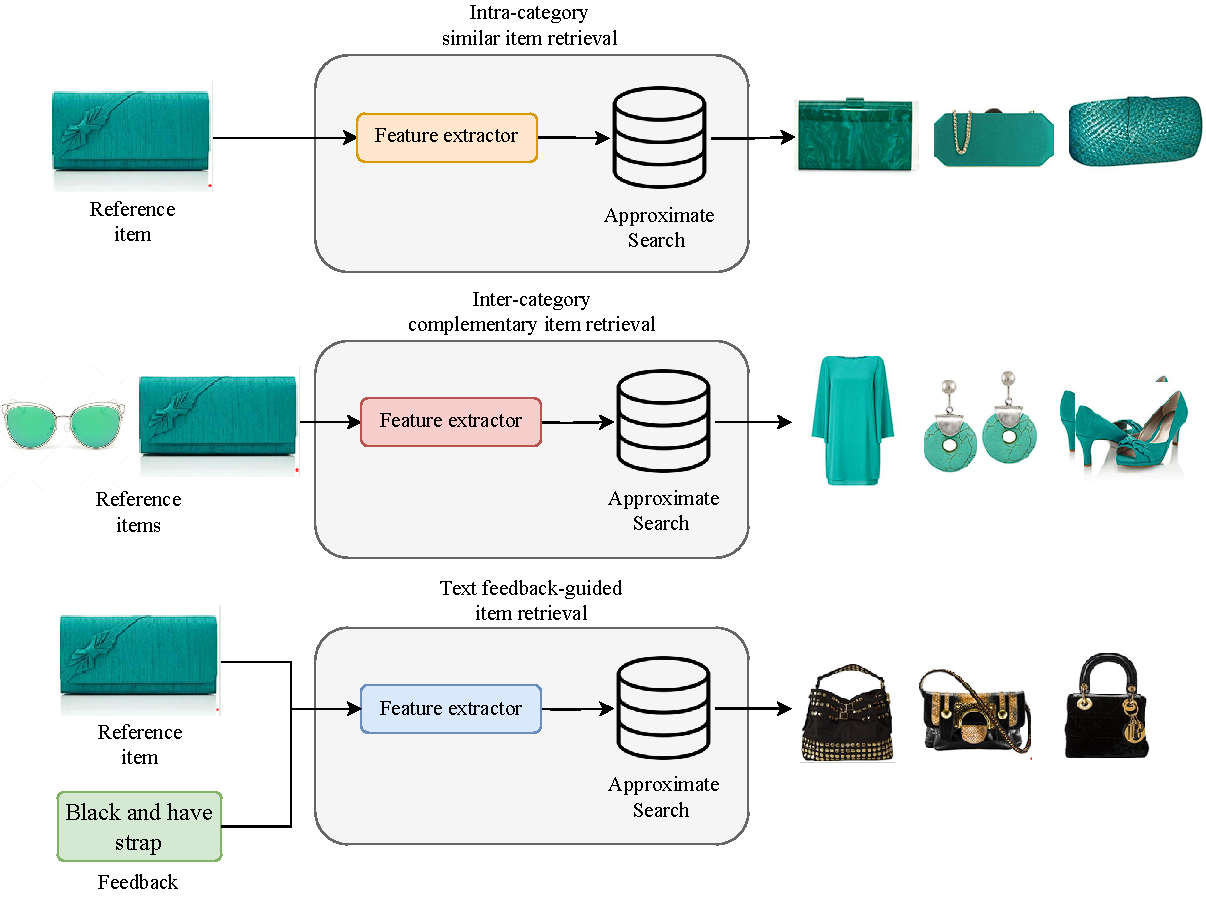
\includegraphics[width=\linewidth]{content/resources/images/fashion-recommendation/chapter4-overview.pdf}
    \caption{Our investigation scope on fashion recommendation}
    \label{fig:chapter4-overview}
\end{figure}

The first approach is \textbf{intra-category similar item retrieval}, where we search for items within the same category and with similar visual representations to the reference item. 

The second approach, called \textbf{inter-category complementary item retrieval}, broadens the scope by considering items from different categories that complement the reference item to make a complete outfit. We define a complete outfit as an outfit that contains at most one item of each category, and all items share a similar style or are visually compatible. This approach differs from the fill-in-the-blank task described in PolyvoreOutfits~\cite{Mariya-ECCV18-Learning}, where each outfit has only one missing item. Our problem is more generalized, allowing for varying numbers of missing items in an outfit.
The last approach we investigate in this thesis is \textbf{text feedback-guided item retrieval}. In this approach, we aim to find fashion items that satisfy the constraints expressed in the user's feedback, provided in natural language. The feedback may describe relative attributes such as being more formal or having longer sleeves.  

In all mentioned approaches, after extracting the visual features of the desired items, we utilize the PolyvoreOutfits dataset~\cite{Mariya-ECCV18-Learning} and search through the embedded features of all items to find the most similar ones. This dataset contains metadata for 251,008 fashion items, and 35,140 outfits, and covers 11 categories: bags, tops, outerwear, hats, bottoms, scarves, jewelry, accessories, shoes, and sunglasses. Due to the dataset's scale, we explore the use of approximate search methods \cite{Sivic-ICCV2003-Video, Erik-Github-Annoy, Malkov-TPAMI2018-Efficient} instead of the commonly used exhaustive K-Nearest Neighbor method for more efficient searching. \autoref{fig:chapter4-overview} illustrates our investigation scope on fashion recommendation.

\begin{figure}[b]
    \centering
    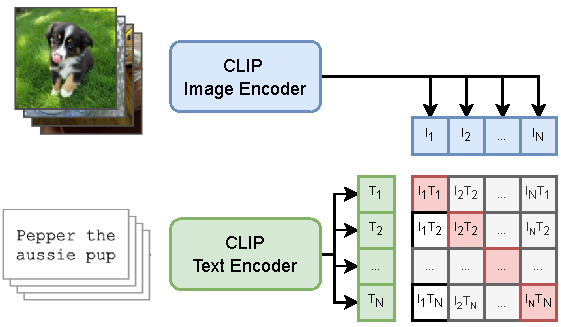
\includegraphics{content/resources/images/fashion-recommendation/chapter4-clip.pdf}
    \caption{CLIP learning process}
    \label{fig:chapter4-clip}
\end{figure}

\section{Dataset Preprocessing}
As we use the visual features of items in the dataset in every search, we extract the visual embedding of all items beforehand and use them directly in later searches. In this thesis, we utilize CLIP~\cite{Radford-OpenAIblog2019-Language}, which learns joint representations of images and their corresponding textual descriptions (\autoref{fig:chapter4-clip}), to encode all items. Both the Image and Text Encoder of CLIP are built upon the Transformer Encoder~\cite{Vaswani-NeurIPS2017-Attention} block. By passing an image through the CLIP model, we obtain a visual embedding that captures its visual features and semantic information.


\section{Intra-category Similar Item Retrieval}
In terms of intra-category similar item retrieval, we first extract the visual embeddings of the reference image using the same CLIP model that we used to extract the embeddings of all items in our dataset. Subsequently, the approximate searching algorithm uses the extracted features to retrieve similar items from the PolyvoreOutfits dataset. \autoref{fig:chapter4-similar} illustrates our similar item retrieval pipeline.

\begin{figure}[h!]
    \centering
    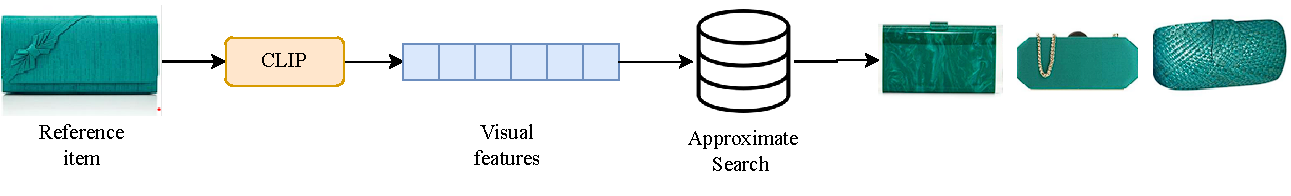
\includegraphics[width=\linewidth]{content/resources/images/fashion-recommendation/chapter4-similar.pdf}
    \caption{Similar item retrieval pipeline}
    \label{fig:chapter4-similar}
\end{figure}

\section{Inter-category Complementary Item Retrieval}
We address the inter-category complementary item retrieval task as the sentence generation task in the natural language domain. Transformers~\cite{Vaswani-NeurIPS2017-Attention}, a deep learning architecture for natural language processing (NLP) tasks, has proven its efficiency in generating a complete sentence from some given keywords~\cite{bhatia-github-keytotext} or a partial sentence~\cite{Devlin-ArXiv2018-BERT}.

In this thesis, we investigate using the Transformers architecture to retrieve complementary items and make a complete outfit. We name this method \textbf{O}utfit \textbf{R}etrieval \textbf{T}ransformers (ORT). Specifically, we consider a complete outfit as a sequence of fashion items, where the order is determined by their categories: bags, tops, outerwear, hats, bottoms, scarves, jewelry, accessories, shoes, and sunglasses. Not all categories are required. All items in an outfit are divided into three groups: \textit{Input}, \textit{Output}, and \textit{Unavailable}. The division of items among these groups depends on whether it's the training or inference phase.

PolyvoreOutfits~\cite{Mariya-ECCV18-Learning} dataset provides us with the metadata of over 35,000 complete outfits, including which items belong to each outfit. Thus, in the training phase, we divide items into an outfit as follows:
\begin{itemize}
    \item \textit{Input} items are selected randomly from the available items.
    \item The remaining items within available items are \textit{Outfit} items.
    \item Items in categories that the outfit lacks are denoted as \textit{Unavailable}.
\end{itemize}

During the inference phase, as we generate complementary items for the reference item, we use the following division:
\begin{itemize}
    \item \textit{Input} item is the reference item only.
    \item \textit{Output} items belong to categories that we aim to propose to users. These items are our target complementary items.
    \item Items in the remaining categories are denoted as \textit{Unavailable}.
\end{itemize}

Each group of items has different ways to represent their embedding:
\begin{itemize}
    \item \textit{Input}: the item's visual embedding as-is.
    \item \textit{Output}: a shared, learnable embedding, denoted as \textit{<OUT>}.
    \item \textit{Unavailable}: a shared, learnable embedding, denoted as \textit{<UN>}.
\end{itemize}

\begin{figure}[h!]
    \centering
    \subfloat[Train phase]{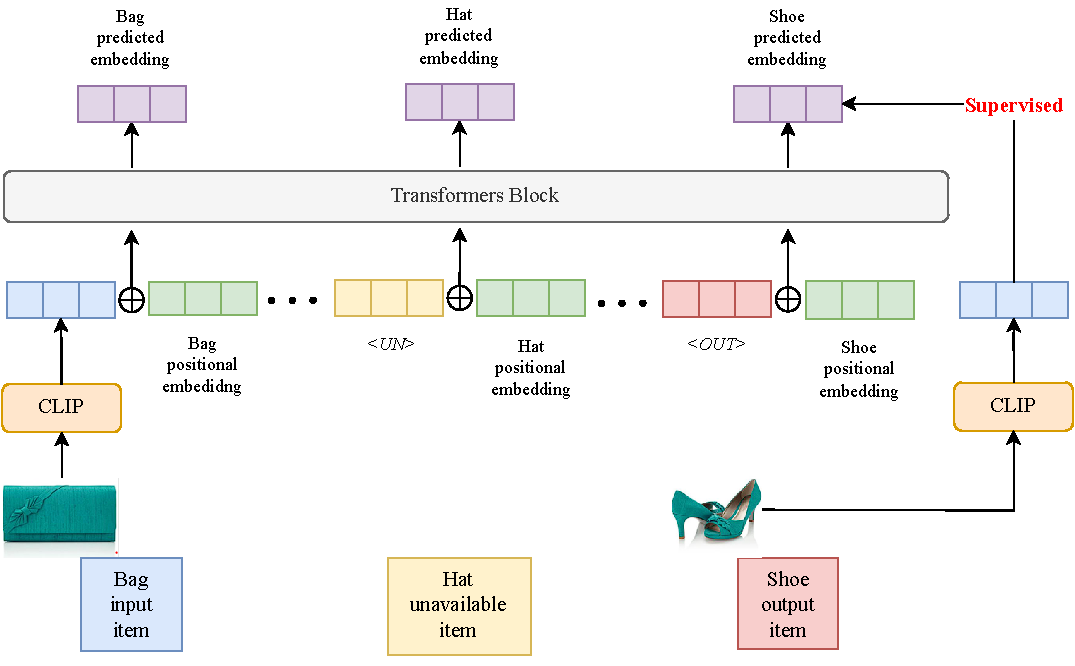
\includegraphics[width=\linewidth]{content/resources/images/fashion-recommendation/chapter4-comp-train.pdf}}
    \hspace{0.5cm}
    \subfloat[Inference phase]{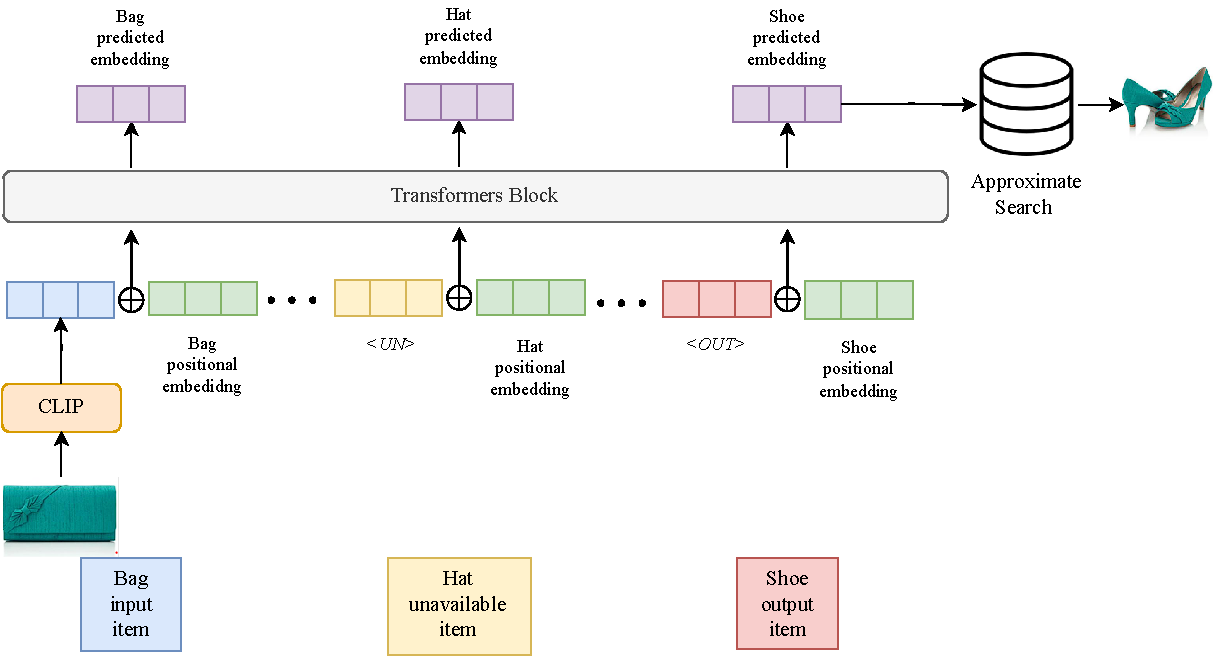
\includegraphics[width=\linewidth]{content/resources/images/fashion-recommendation/chapter4-comp-test.pdf}} 
    \caption{Outfit Retrieval Transformers pipeline.}
    \label{fig:chapter4-outfit-trans}
\end{figure}

All embeddings are fed into a Transformers Encoder block~\cite{Vaswani-NeurIPS2017-Attention} to produce cross-semantic-aware output embeddings (as shown in \autoref{fig:chapter4-outfit-trans}). ORT also use positional embeddings technique~\cite{Vaswani-NeurIPS2017-Attention}, where each position specifies the item's category. During the training phase, the network minimizes the noise contrastive loss~\cite{Lai-Arxiv2019-Contrastive} so the Transformers block learns to maximize the similarity between its output embeddings and the \textit{Output} items' original visual embeddings (as shown in \autoref{fig:chapter4-outfit-trans}(a)). We formulate the loss $L$ as follows:
\begin{align}
    & L = -\frac{1}{N}*\Sigma_{i=1}^{N} log{\frac{exp(S_{i_P})}{exp(S_{i_P}) + exp(S_{i_N})}},\\
    & S_{i_P} = cos(pred_i, pos_i),\\
    & S_{i_N} = \Sigma_{j \in {neg_i}} cos(pred_i, j),
\end{align}

where $N$ is the number of \textit{Output} items in all outfits, $pred_i$ is the $i^{th}$ predicted output embeddings, $pos_i$ is the ground-truth visual embeddings of that \textit{Output} item, $neg_i$ is a set of negative samples which contains the embeddings of other items of the same category. 

During the inference phase, we utilize the approximate searching algorithm to retrieve similar items from ORT's output embeddings (as shown in \autoref{fig:chapter4-outfit-trans}(b)).

\section{Text Feedback-guided Item Retrieval}
To address this task, we adopt the CLIP4Cir architecture proposed by Baldrati et al~\cite{Baldrati-CVPR2022-Conditioned}. The architecture proves efficiency despite its simplicity. It first utilizes CLIP model~\cite{Radford-OpenAIblog2019-Language} to extract embeddings from both the reference image and relative feedback. Then, both embeddings are fed into a Combiner network, a small trainable network specifically designed to merge the two embeddings into a single output embedding (as shown in \autoref{fig:chapter4-combiner}).

\begin{figure}[t!]
    \centering
    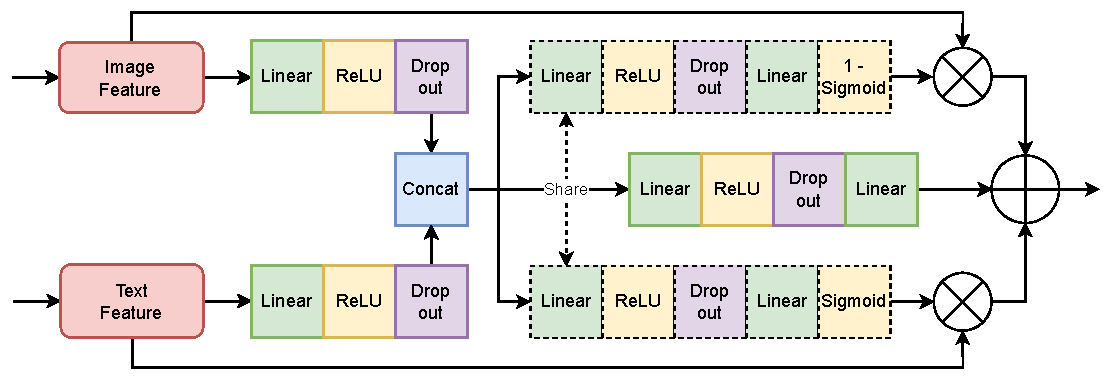
\includegraphics[width=\linewidth]{content/resources/images/fashion-recommendation/chapter4-combiner.pdf}
    \caption{Combiner architecture}
    \label{fig:chapter4-combiner}
\end{figure}


\begin{figure}[t!]
    \centering
    \subfloat[Train phase]{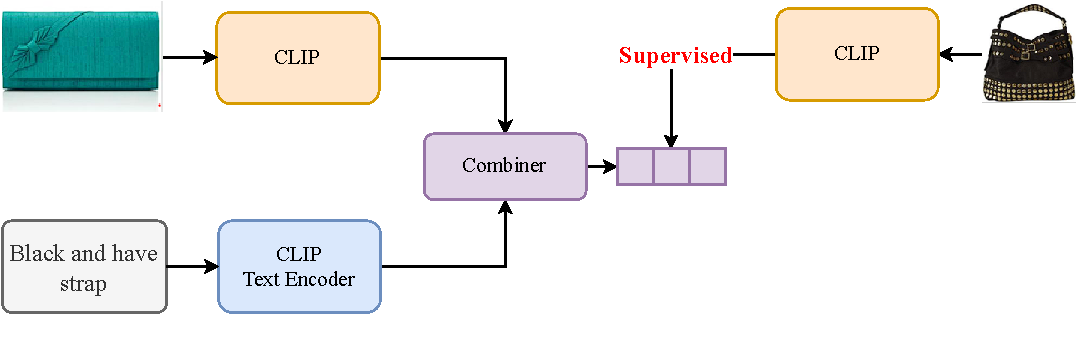
\includegraphics[width=0.85\columnwidth]{content/resources/images/fashion-recommendation/chapter4-clip4cir-train.pdf}}
    \hspace{0.5cm}
    \subfloat[Inference phase]{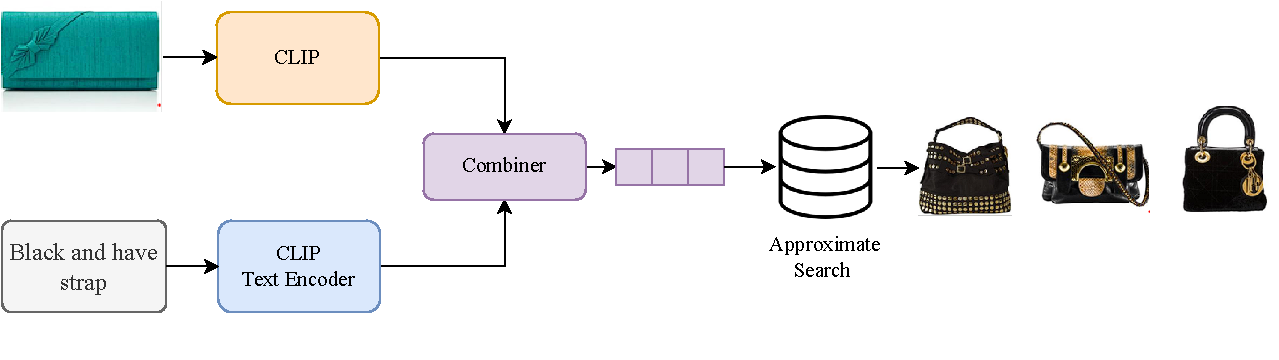
\includegraphics[width=\columnwidth]{content/resources/images/fashion-recommendation/chapter4-clip4cir-test.pdf}} 
    \caption{CLIP4Cir pipeline.}
    \label{fig:chapter4-clip4cir}
\end{figure}

During the training phase, we utilize the FashionIQ dataset~\cite{Wu-CVPR2021-FashionIQ}, which consists of triplet pairs comprising a reference image, relative feedback, and a target image. The Combiner is trained to maximize the similarity between its output embeddings and the target images' embeddings produced by CLIP (\autoref{fig:chapter4-clip4cir}(a)), specified by the following symmetric contrastive loss $L$:
\begin{align}
    & L = \frac{1}{2}(L_c + L_i),\\
    & L_c = \text{cross\_entropy\_loss}(E_cE_i, logits),\\
    & L_i = \text{cross\_entropy\_loss}(E_iE_c, logits),
\end{align}

where $logits$ denotes the list $\{1, 2, ..., N\}$ with $N$ is the batch size, $E_c$ denotes a batch of Combiner's output embeddings and $E_i$ denotes a batch of CLIP's output embeddings. This shared representation space allows us to effectively compare the similarity between the embeddings produced by the Combiner and CLIP.

To run inference, we also leverage the approximate searching algorithm to retrieve similar items for the target output embeddings (as shown in \autoref{fig:chapter4-clip4cir}(b)).

\section{Approximate Searching}
In all of the three recommendation approaches we have investigated so far, the final involves retrieving the items from the dataset that have visual embeddings most similar to a given input embedding.

For such nearest neighbor problem, K-Nearest Neighbor (KNN) algorithm are widely used due to its simplicity and giving exact results(\cite{Lin-CVPR2020-Fashion, Baldrati-CVPR2022-Conditioned, Baldrati-CVPR2022-Effective, Sarkar-CVPRW2022-OutfitTransformer}.  The KNN algorithm exhaustively searches through every dimension of all items in the dataset. As a result, this algorithm has the runtime complexity of $O(kNd)$ where $k$ is the number of items to retrieve, $N$ is the size of the dataset, and $d$ is the number of dimensions to represent one item, in our case, it is the length of the visual embedding produced by CLIP~\cite{Radford-OpenAIblog2019-Language}. 

Approximate searching algorithms solve this problem by lowering either $N$ or $d$, thus allowing the search faster with the accuracy trade-off. Approximate methods also help compress the dataset due to the decline of $d$~\cite{Gionis-VLDB1999-Similarity, Jegou-TPAMI2010-Product}. However, as mentioned in Jegou's work~\cite{Jegou-ICASSP2011-IVFPQ}, these methods significantly decrease the result accuracy.  In this thesis, our primary goal is to find the fastest approximate methods while keeping a reasonable accuracy. Thus, we focus on investigating three common algorithms that lower the search space $N$: Inverted File Index~\cite{Sivic-ICCV2003-Video} (IVF), Hierarchical Navigable Small Worlds~\cite{Malkov-TPAMI2018-Efficient} (HNSW), and Approximate Nearest Neighbors Oh Yeah~\cite{Erik-Github-Annoy} (ANNOY). We use the Euclidean metric as our distance metric while retrieving nearest neighbors.

\subsection{Inverted File Index (IVF)}
The basic idea behind the Inverted File Index~\cite{Sivic-ICCV2003-Video} is to partition the dataset into multiple subsets, usually done by employing K-Means. We denote the number of subsets as $nlist$. Subsequently, all embeddings in the dataset are stored separately in their corresponding subset. Each subset also contains a centroid, which is the mean of all embeddings in that subset. 

We calculate the distance between the input embedding and all centroids during the query process and take the closest one. Then, we only search through all items in the corresponding subset. This means the larger $nlist$, the smaller subset we need to search through. 

\begin{figure}[h!]
    \centering
    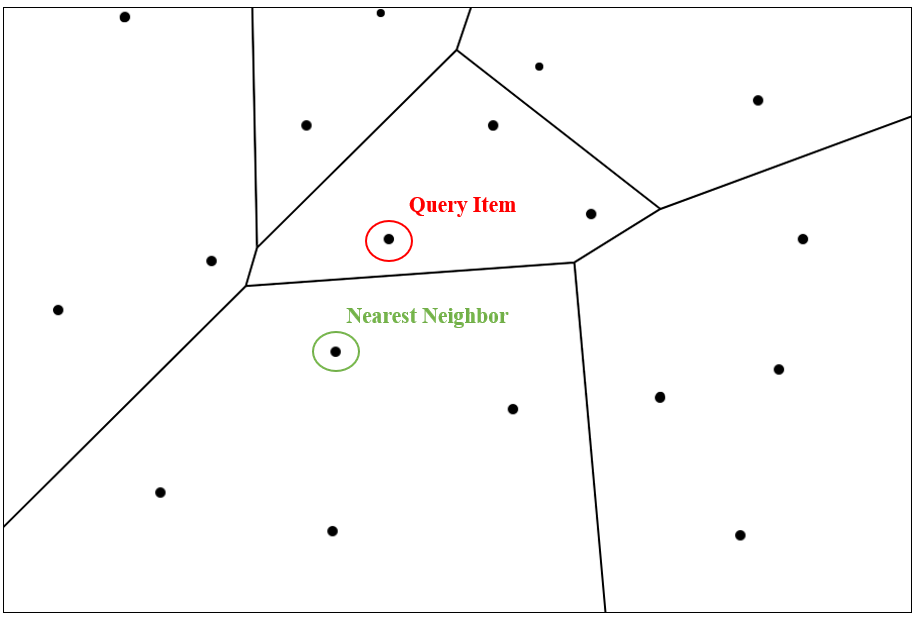
\includegraphics[width=0.7\linewidth]{content/resources/images/fashion-recommendation/chapter4-ivf.png}
    \caption{The case where the query embedding falls on the outskirts of the closest subset in IVF}
    \label{fig:chapter4-ivf}
\end{figure}

However, if the query embedding falls on the outskirts of the closest subset, its nearest neighbors may belong to nearby clusters (\autoref{fig:chapter4-ivf}). This is what makes this method approximate and not exact. The impact can be reduced by searching for multiple nearby subsets; we denote the number of subsets to search as $nprobe$. A larger $nprobe$ means taking more time but giving better accuracy. The number of subsets $nlist$ and the number of subsets to search $nprobe$ can be tuned to find the time/accuracy reasonable trade-off. 

\subsection{Approximate Nearest Neighbors Oh Yeah (ANNOY)}
ANNOY~\cite{Erik-Github-Annoy} is the search algorithm used by Spotify in their music recommendation system~\cite{Erik-Github-Annoy}. The key idea of ANNOY is to build a binary tree, where each leaf node is an item in the dataset. ANNOY selects a random hyperplane to partition the dataset into two subsets at each intermediate node in the tree construction process. This hyperplane is determined by sampling two random points from the corresponding subset and taking the hyperplane equidistant from them. The construction process is shown in \autoref{fig:chapter4-annoy}. The constructed tree structure is stored alongside the dataset.

\begin{figure}[thb!]
    \centering
    \subfloat[Construction process]{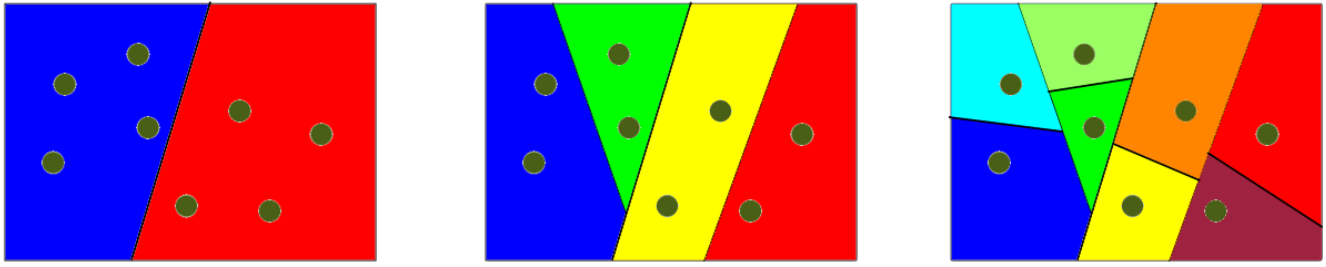
\includegraphics[width=0.9\columnwidth]{content/resources/images/fashion-recommendation/chapter4-annoy-step.png}}
    \hspace{0.1mm}
    \subfloat[Constructed tree]{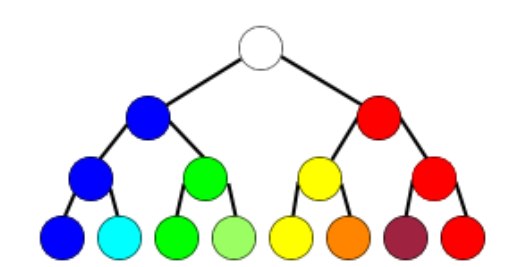
\includegraphics[width=0.5\columnwidth]{content/resources/images/fashion-recommendation/chapter4-annoy-tree.png}} 
    \caption{ANNOY index construction process}
    \label{fig:chapter4-annoy}
\end{figure}

We traverse the binary tree from the root during the query process by repeatedly checking which side of the corresponding hyperplane the query embedding belongs to.
This method also faces the same issue as IVF; if the query item falls on the outskirts of a subspace, the nearest neighbors may appear in sibling leaf nodes instead. To tackle this problem, ANNOY allows searching for multiple leaf nodes, which can be done by using a priority queue to keep track of the closest hyperplane so we can backtrack to that hyperplane and go to the other side. ANNOY also proposes building multiple trees at once to minimize the effect of randomness. 

We denote the number of trees to build as $n\_{trees}$ and the total number of leaf nodes to search in all trees as $search\_k$. A larger $n\_{trees}$ gives more accurate results but larger memory usage; it does not affect the query time. A larger $search\_k$ leads to more accurate results but longer query time.

\subsection{Hierarchical Navigable Small Worlds (HNSW)}
The key idea of Hierarchical Navigable Small Worlds~\cite{Malkov-TPAMI2018-Efficient} (HNSW) is taken from the Skip List data structure. Skip List is a data structure that consists of multiple sorted linked lists. The bottom level (or level 0) is the ordinary linked list containing all the elements. The higher levels contain fewer elements and act as shortcuts to traverse the list quickly. \autoref{fig:chapter4-skiplist} illustrates the Skip List data structure.

\begin{figure}[th!]
    \centering
    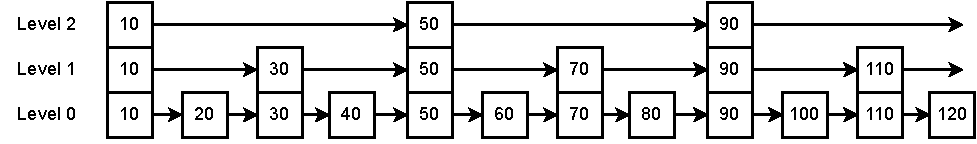
\includegraphics[width=\linewidth]{content/resources/images/fashion-recommendation/chapter4-skiplist.pdf}
    \caption{Skip list data structure}
    \label{fig:chapter4-skiplist}
\end{figure}

To search in a Skip List, we start at the highest level, which has the longest step between elements and iterate towards the end of that level. If the current element is greater than the search value, we move down to the previous node in the \textit{below} level. This process repeats until we find the search value or reach the lowest level (level 0) (as shown in \autoref{fig:chapter4-skiplist-search}).

\begin{figure}[th!]
    \centering
    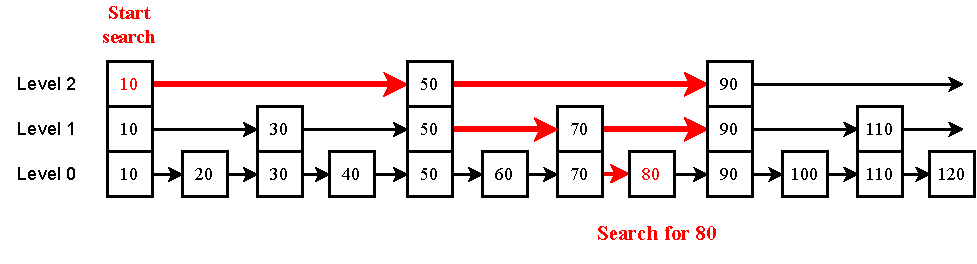
\includegraphics[width=\linewidth]{content/resources/images/fashion-recommendation/chapter4-skiplist-search.pdf}
    \caption{Skip list search process}
    \label{fig:chapter4-skiplist-search}
\end{figure}

HNSW borrows that idea and applies it in higher dimensions. Specifically, HNSW constructs multiple undirected graphs, where the graph at the lowest level (level 0) contains all dataset items as its nodes. The higher-level graphs contain fewer nodes, leading to longer distances between each node. To reduce the number of adjacent nodes during traversing, HNSW limits the maximum degree of each node in all graph levels, denoted as $M$. The HNSW data structure is constructed from a dataset by inserting each embedding vector one by one. Given $M$ is the maximum degree of each node, $efConstruction$ and $efSearch$ are the maximum numbers of nodes to traverse at each level in the index and query process, respectively, the steps to insert a new embedding vector are as follows:
\begin{enumerate}
    \item If this is the first item, insert it to all levels and continue.
    \item Find the graph level $L$ to insert the new item. The value of $L$ has exponentially decreasing probability as it goes higher, specified by the equation $L = max(floor(-log(uniform(0, 1))), log(M))$. This also means the max level $L_{max}$ is $log(M)$.
    \item From level $L_{max}$ down to $L + 1$, we repeatedly find the nearest embedding from the entry point (the first inserted item for level $L_{max}$) and use that embedding as the entry point for the next level.
    \item From level $L$ down to $0$, we repeatedly find $efConstruction$ nearest embeddings from the entry point. Subsequently, we calculate the distance between the input embedding and those embeddings to find the nearest $M$ and link the input embedding to them. We use the nearest embedding out of $M$ as the entry point for the next level.
\end{enumerate}

\begin{figure}[th!]
    \centering
    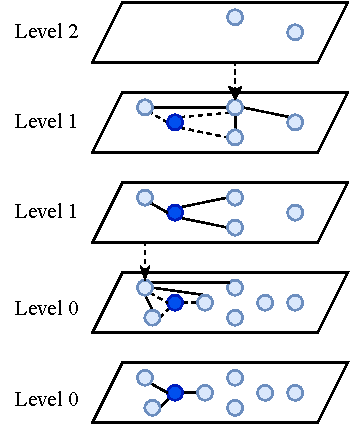
\includegraphics[width=0.5\linewidth]{content/resources/images/fashion-recommendation/chapter4-hnsw-create.pdf}
    \caption{Insert a new vector into HNSW at level 1}
    \label{fig:chapter4-hnsw-create}
\end{figure}

\autoref{fig:chapter4-hnsw-create} illustrates the steps to insert a new item into HNSW, given $M = 3$ and $efConstruction = 4$. 

Regarding the query process of HNSW, from level $L_{max}$, we repeatedly find the nearest embeddings from the entry point and use that embedding as the entry point for the next level. Upon entering level 0, we find $efSearch$ nearest embeddings and compare the query embedding with each of them to get the nearest one. A higher $efSearch$ takes longer query time but gives more accurate results. The search process is greedy, and thus cannot ensure exact results.

\section{Experiments}
\subsection{Detailed Implementation}

For intra-category similar item retrieval, we employed the pretrained CLIP model released by Baldrati et al.~\cite{Baldrati-CVPR2022-Conditioned} to extract the visual embeddings of the reference image and all items in the dataset.

For inter-category complementary item retrieval, the Outfit Retrieval Transformers (ORT) block has 6 layers, 8 attention heads, and 11 inputs in total (same as the number of categories of PolyvoreOutfits), and each input has 640 dimensions (same as CLIP output dimension). We trained the network from scratch on the PolyvoreOutfits dataset~\cite{Mariya-ECCV18-Learning}. The AdamW optimizer was used with a learning rate 0.0001 and a weight decay of 0.3. The learning rate scheduler had a step size of 20 with a gamma factor 0.5. 

For text feedback-guided item retrieval, we utilized the pretrained CLIP and Combiner models released by Baldrati et al.~\cite{Baldrati-CVPR2022-Conditioned} to extract both the visual and textual embeddings from inputs and produce the merged output.

In terms of approximate search, we used the FAISS~\cite{johnson-bigdata2019-faiss} implementation for IVF and HNSW algorithms, and the official implementation~\cite{Erik-Github-Annoy} of ANNOY algorithm. 

\subsection{Intra-category similar item retrieval evaluation}
We performed a zero-shot evaluation on the DeepFashion dataset~\cite{Liu-CVPR2016-DeepFashion}, without fine-tuning the CLIP model on it.
This dataset contains 14,812 query images and 12,612 test images. Each image is assigned a label, and the dataset has a total of 8,082 unique labels.

For evaluation, we used the recall at rank K metric, with K in the list $\{1, 5, 10, 30, 50\}$.
Specifically, we retrieved K images from the test set using the KNN algorithm for each query image. 
We considered the query correct if any of the K retrieved images had the same label as the query image.
The recall score was calculated by dividing the number of correct queries by the total number of query images and multiplying the result by 100.
The evaluation results are shown in \autoref{table:chapter4-zero-shot}.
In a zero-shot evaluation, these results are acceptable.
As we see in \autoref{fig:chapter4-similar-sample}, the false recommendations still look relevant to the reference images. 

\begin{table}[h!]
\centering
\begin{tabular}{l c c c c c}
\hline
& R@1  & R@5 & R@10 & R@30  & R@50         \\ \hline
Zero-shot CLIP~\cite{Baldrati-CVPR2022-Conditioned}  & 13.13  & 31.62 & 43.55 & 60.25  & 68.04           \\ \hline
\end{tabular}
\caption{Recall at rank K (R@K) of zero-shot CLIP on the DeepFashion dataset}
\label{table:chapter4-zero-shot}
\end{table}

\begin{figure}[h!]
    \centering
    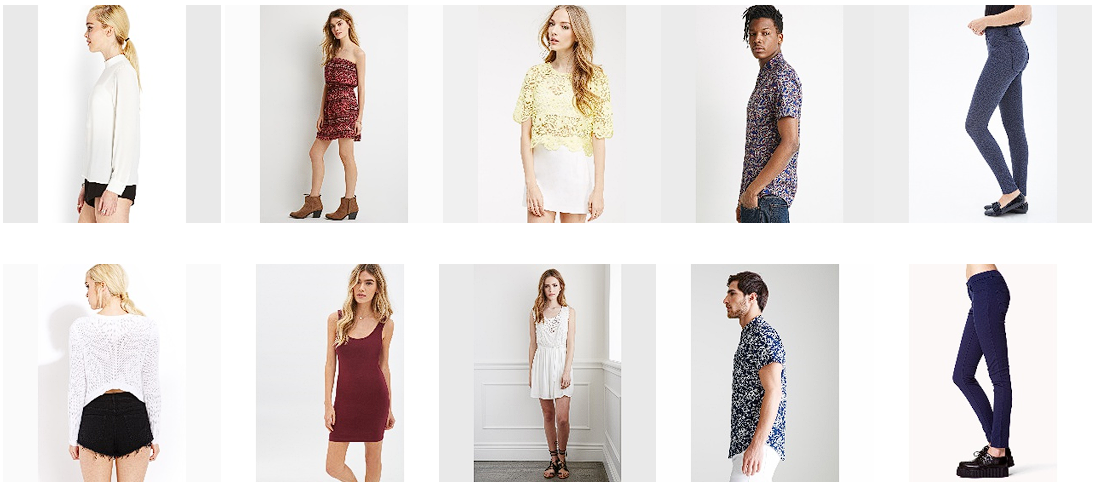
\includegraphics[width=0.75\linewidth]{content/resources/images/fashion-recommendation/chapter4-similar-sample.PNG}
    \caption{Some false recommendation in similar item retrieval evaluation. Top: reference image. Bottom: top 1 result}
    \label{fig:chapter4-similar-sample}
\end{figure}

\subsection{Inter-category complementary item retrieval evaluation}
We performed the evaluation on the PolyvoreOutfits dataset~\cite{Mariya-ECCV18-Learning} for this task.
This dataset includes 251,008 fashion items, classified into 11 distinct categories.
The distribution of items across these categories is shown in \autoref{fig:polyvore-cate}.

\begin{figure}[h!]
    \centering
    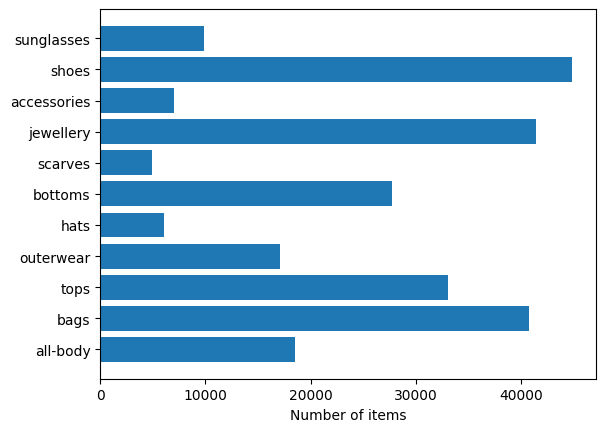
\includegraphics[width=0.6\linewidth]{content/resources/images/fashion-recommendation/chapter4-polyvore-cate.png}
    \caption{Number of items of each category in PolyvoreOutfits}
    \label{fig:polyvore-cate}
    \vspace{-2mm}
\end{figure}

Additionally, PolyvoreOutfits contains the metadata of 35,140 outfits. Each outfit in the dataset follows the constraint of including at most one item from each category. As a result, the number of items within each outfit can range from 2 to 11.
\autoref{fig:polyoutfit-cate} shows the number of outfits each category appears in the train, validation, and test set.

\begin{figure}[h!]
    \centering
    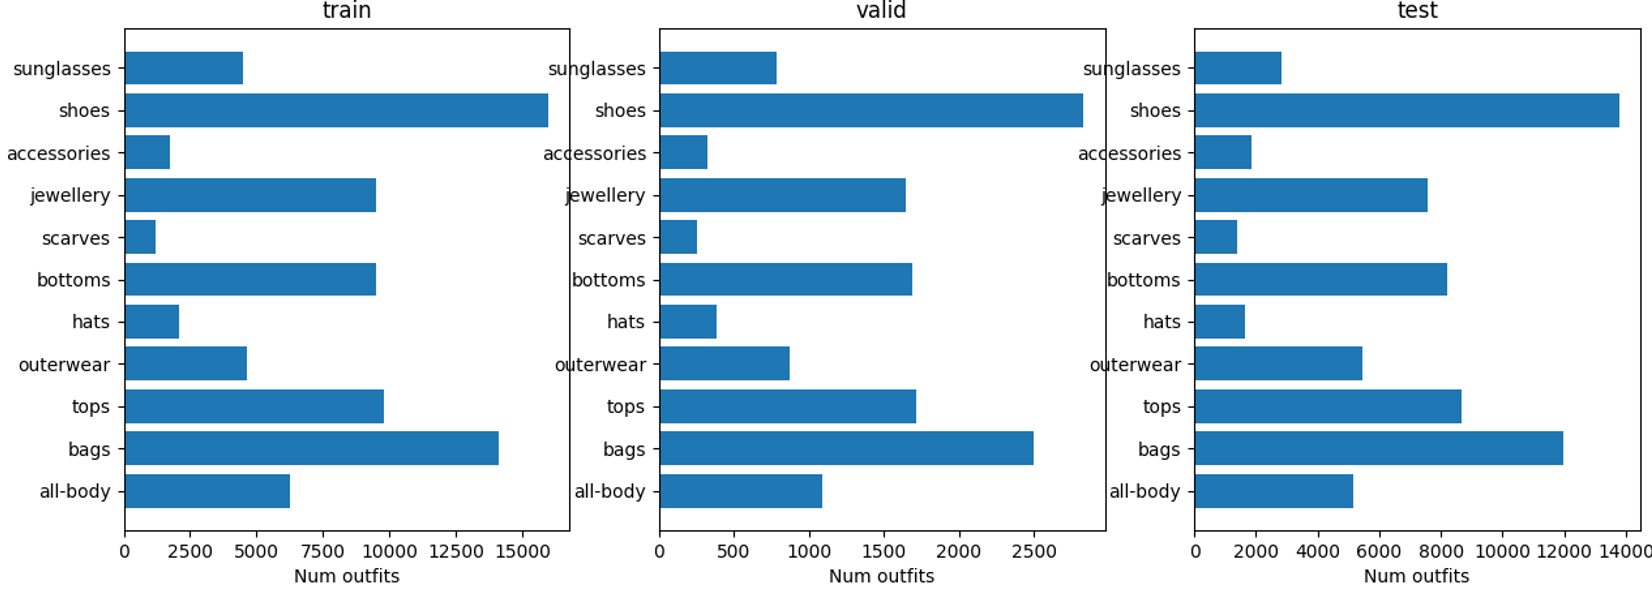
\includegraphics[width=\linewidth]{content/resources/images/fashion-recommendation/chapter4-polyoutfit-cate.png}
    \caption{The number of outfits each category appears in PolyvoreOutfits}
    \label{fig:polyoutfit-cate}
\end{figure}

To fine-tune the Outfit Retrieval Transformers, we utilized the outfits in the validation set. 
The metric for evaluation was the recall at rank K, which was calculated as follows:
\begin{enumerate}
    \item For each \textit{Output} item, retrieve K items within the same category as the original item using KNN. If the retrieved K items contain the original item, mark this \textit{Output} correct.
    \item The recall score equals the number of correct \textit{Output} items divided by the total number of \textit{Output} items and multiplied by 100.
\end{enumerate} 

We investigated various settings and selected the configuration that achieved the highest recall at rank 10. 
The experiments were conducted with the following setups:
\begin{itemize}
    \item Mean squared error loss and noise contrastive loss.
    \item Final loss involves output normalization and does not involve output normalization.
    \item Randomly select 90\%, 50\% and 10\% of items in an outfit as \textit{Input} items.
\end{itemize}

While fine-tuning the loss for Outfit Retrieval Transformer (ORT), the output normalization was included in the final loss and 90\% of items in an outfit were chosen as \textit{Input} items. \autoref{fig:chapter4-mse} shows the recall score of MSE loss in the train and validation set, whereas \autoref{fig:chapter4-contrast} shows the result of noise contrastive loss. MSE loss was faster to converge, but the recall was relatively low, even at a higher recall rank. Meanwhile, the contrastive loss could still converge more and also achieve higher recall. In conclusion, we decided to use noise contrastive loss.

\begin{figure}[ht!]
    \centering
    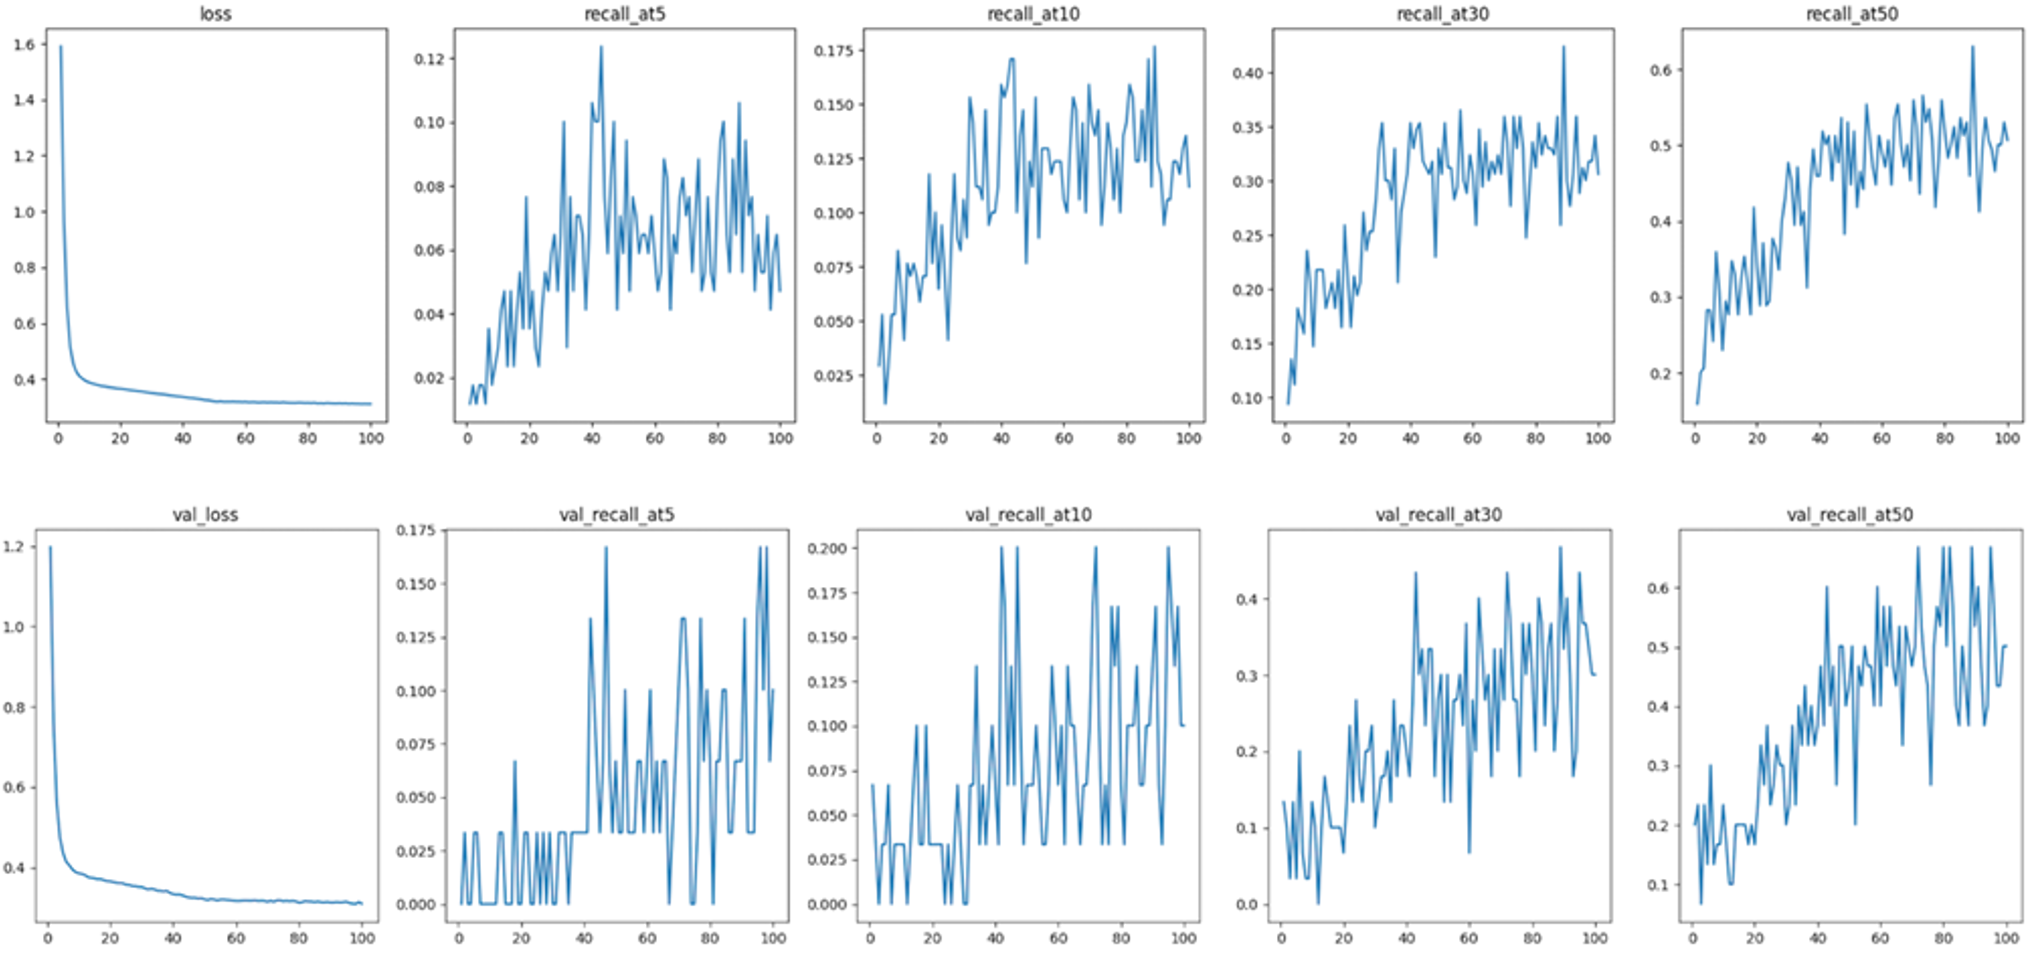
\includegraphics[width=\linewidth]{content/resources/images/fashion-recommendation/chapter4-mse.png}
    \caption{ORT w/ MSE loss. Top: train, bottom: validation}
    \label{fig:chapter4-mse}
\end{figure}

\begin{figure}[ht!]
    \centering
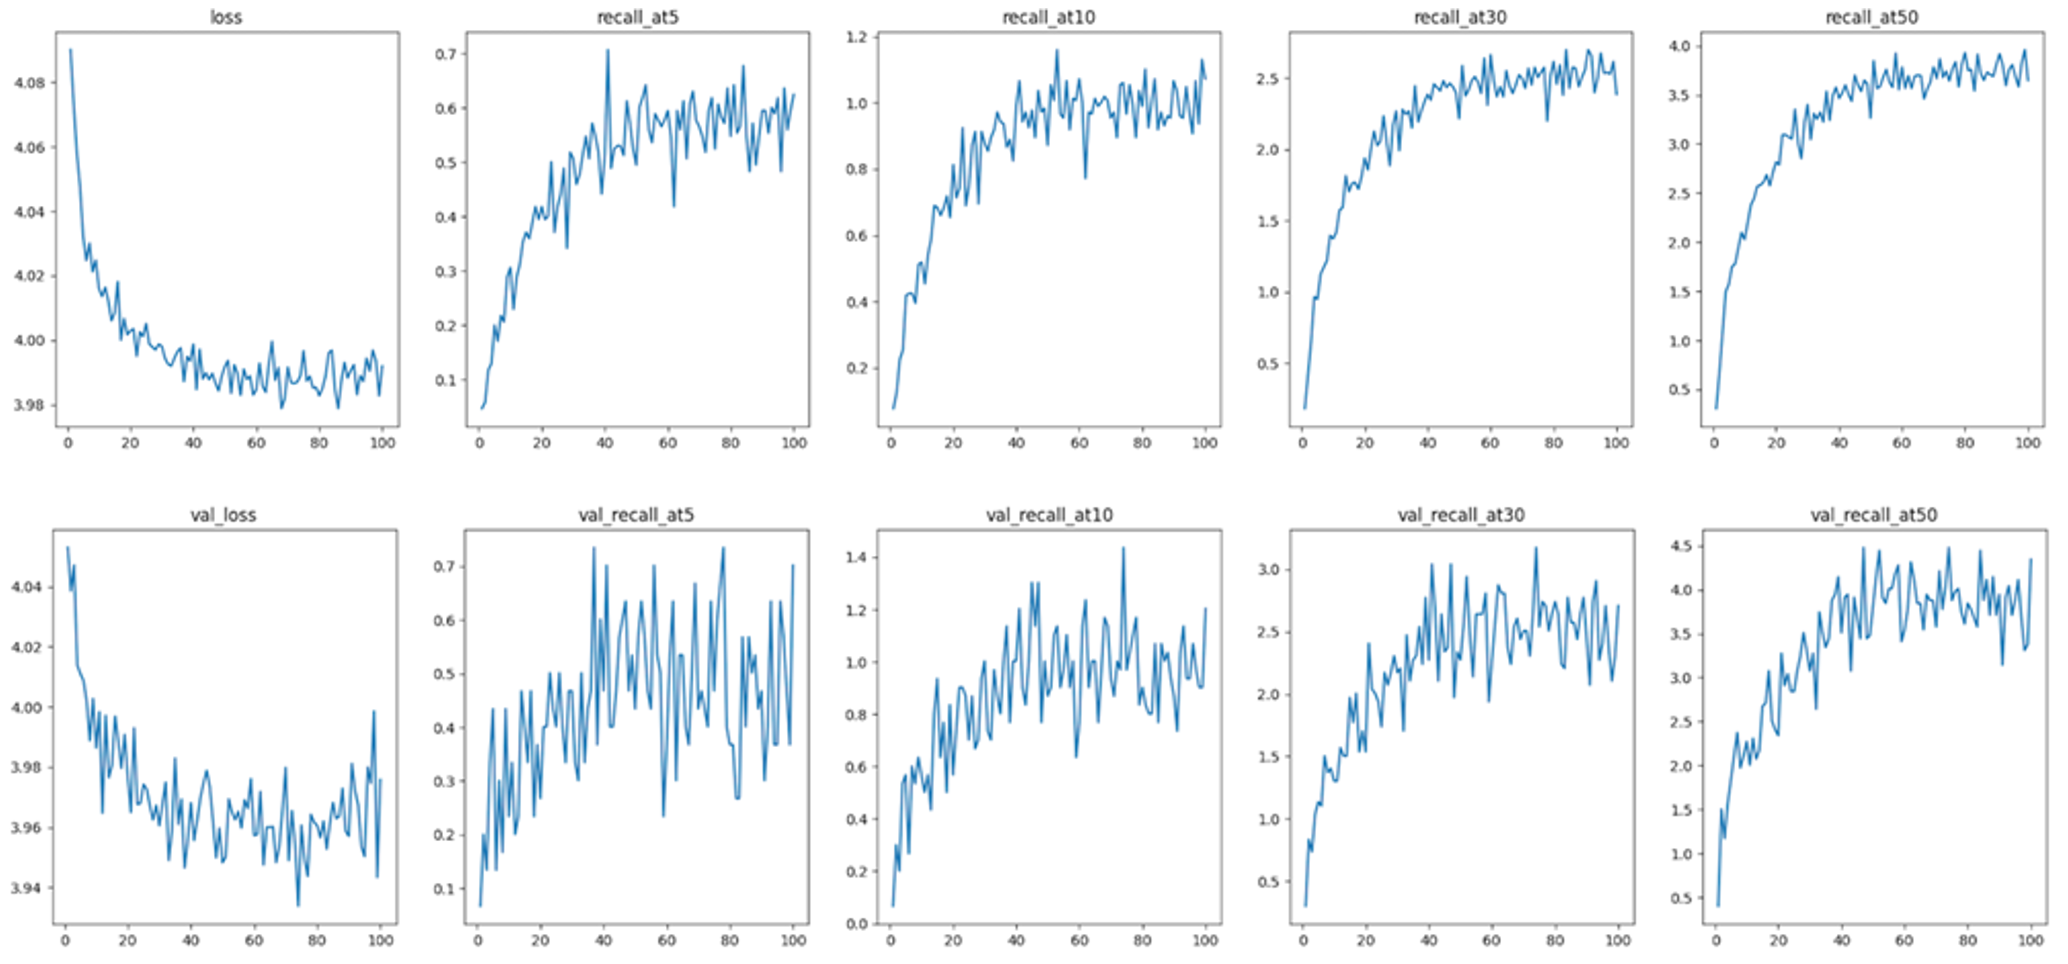
\includegraphics[width=\linewidth]{content/resources/images/fashion-recommendation/chapter4-contrast.png}
    \caption{ORT w/ noise contrastive loss. Top: train, bottom: validation}
    \label{fig:chapter4-contrast}
\end{figure}

We tuned the output normalization using the noise contrastive loss, as they achieved higher results in the above comparison. Moreover, we still kept the \textit{Input} item's percentage at 90\%. \autoref{fig:chapter4-contrast-no-norm} shows the results of not involving output normalizing in the final loss. Compared with \autoref{fig:chapter4-contrast}, we see that we can get higher recall and some signs of overfitting when removing the last output normalization during the training process. However, overall, it still achieves higher recall in both the training and validation set.

\begin{figure}[ht!]
    \centering
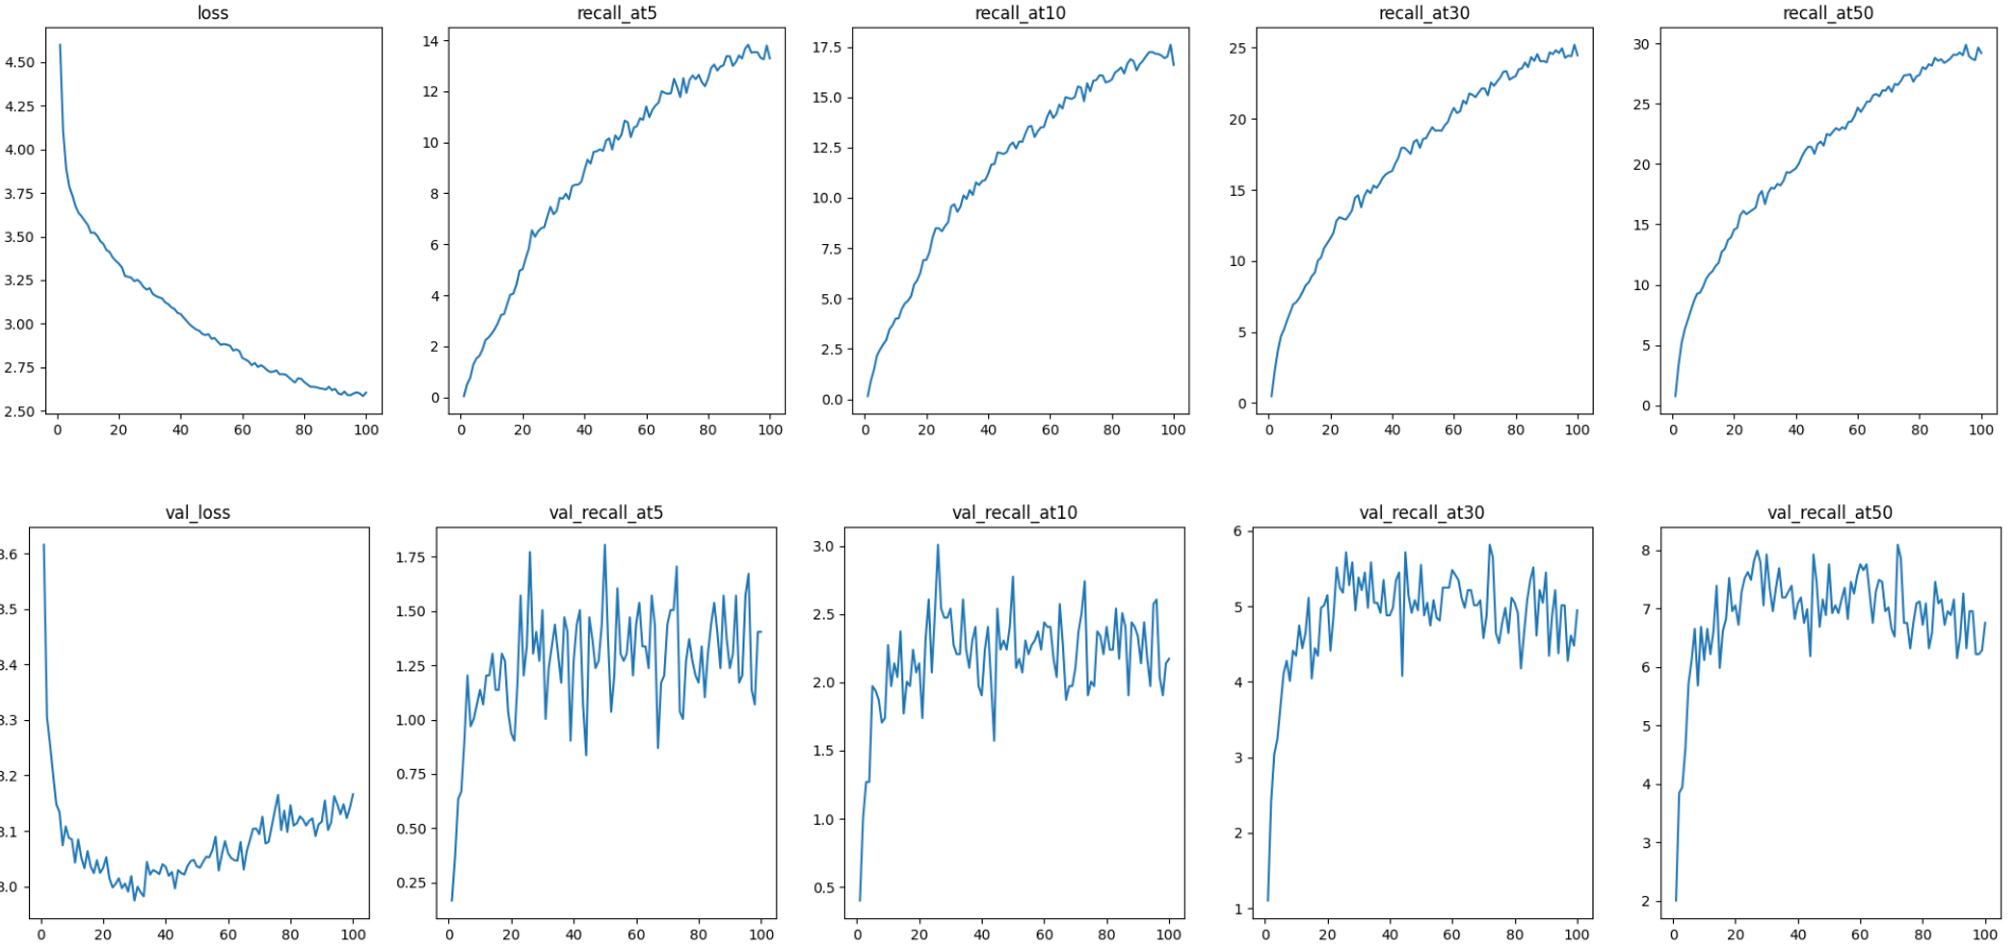
\includegraphics[width=\linewidth]{content/resources/images/fashion-recommendation/chapter4-contrast-no-norm.png}
    \caption{ORT w/o output normalization. Top: train, bottom: validation}
    \label{fig:chapter4-contrast-no-norm}
\end{figure}

\begin{figure}[ht!]
    \centering
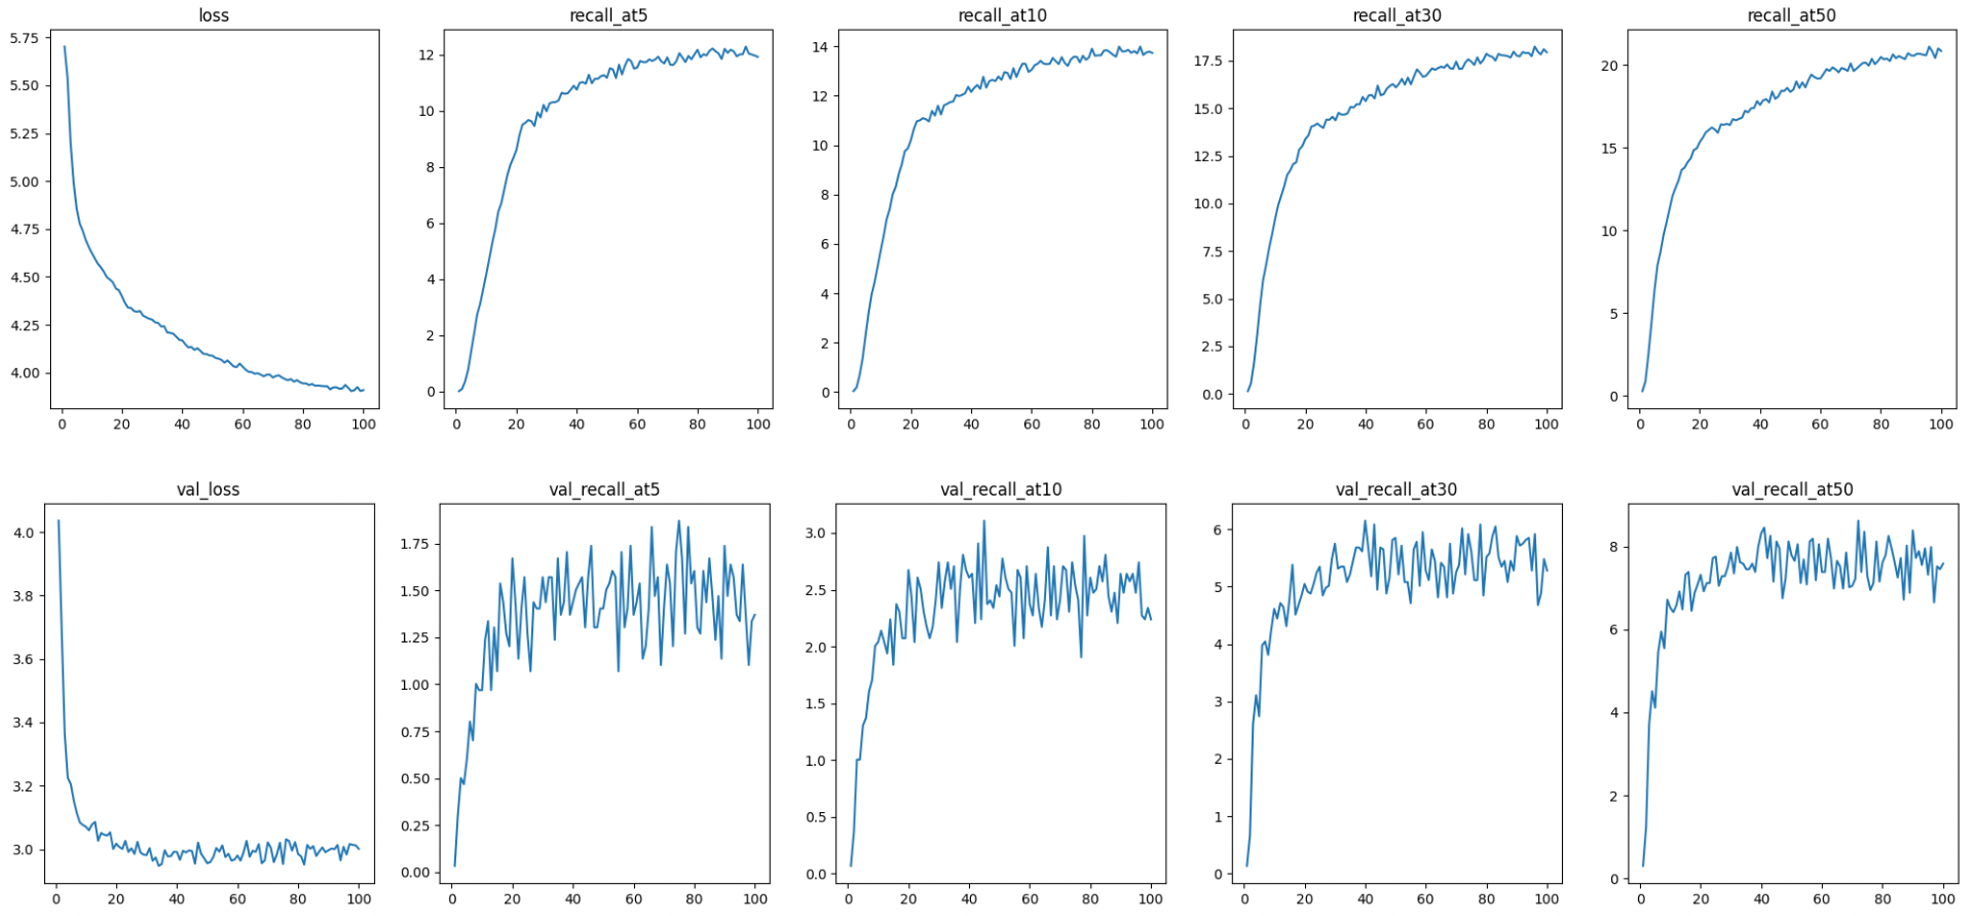
\includegraphics[width=\linewidth]{content/resources/images/fashion-recommendation/chapter4-contrast-no-norm-mask-half.png}
    \caption{ORT w/ 50\% of outfits are \textit{Input} items. Top: train, bottom: validation}
    \label{fig:chapter4-contrast-no-norm-mask-half}
\end{figure}

\begin{figure}[ht!]
    \centering
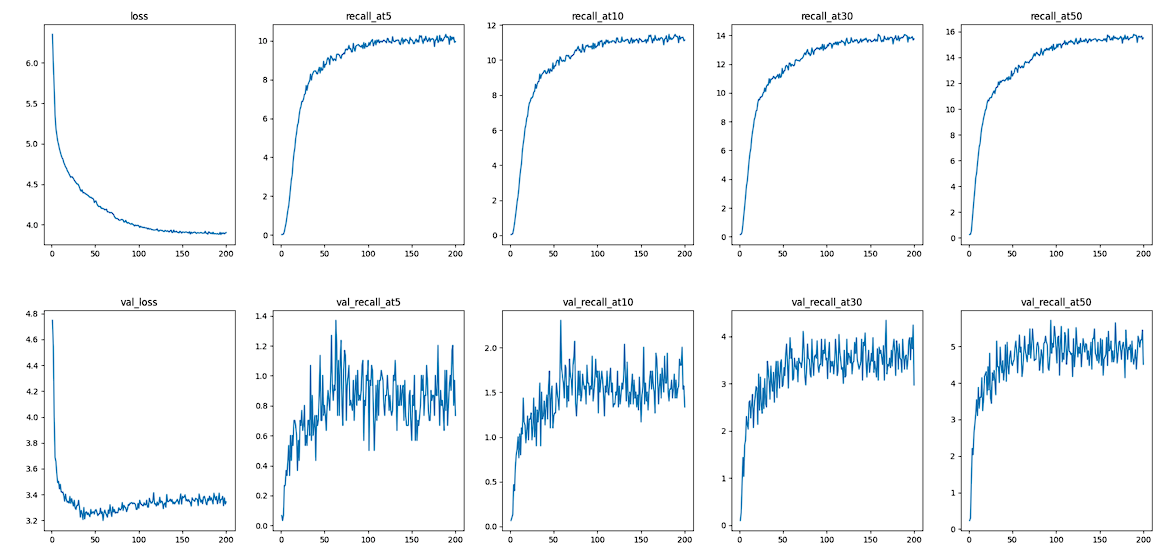
\includegraphics[width=\linewidth]{content/resources/images/fashion-recommendation/chapter4-contrast-no-norm-mask-90.png}
    \caption{ORT w/ 10\% of outfits are \textit{Input} items. Top: train, bottom: validation}
    \label{fig:chapter4-contrast-no-norm-mask-90}
\end{figure}


Using noise contrastive loss and not including output normalization in the final loss, we tuned the \textit{Input} item's percentage in an outfit. \autoref{fig:chapter4-contrast-no-norm-mask-half} shows the situation where 50\% of all outfits are \textit{Input} items in the training phase. Compared with \autoref{fig:chapter4-contrast-no-norm}, the validation recall is still the same as when we only chose 10\% of items, which means the model can learn even with fewer input items. Note that the percentage of \textit{Input} items in the validation set was still kept at 90\%. However, as we decreased the \textit{Input} items percentage to 10\%, the validation recall also dropped significantly (5 in \autoref{fig:chapter4-contrast-no-norm-mask-90} in comparison with 8 in \autoref{fig:chapter4-contrast-no-norm-mask-half}). As a result, we decided to keep the percentage of \textit{Input} items at 50\% % for fine-tuning.

In conclusion, we fine-tuned ORT with noise contrastive loss, no normalization before calculating final loss, and choosing 50\% % of items in an outfit as \textit{Input} items.  
Additionally, We evaluated that model on the test dataset with different mask ratios and recall ranks, as shown in \autoref{fig:chapter4-mask-ratio}. The recall dropped significantly when masking 70\% of the items while slowly dropping when masking fewer items.

\begin{figure}[htb!]
    \centering
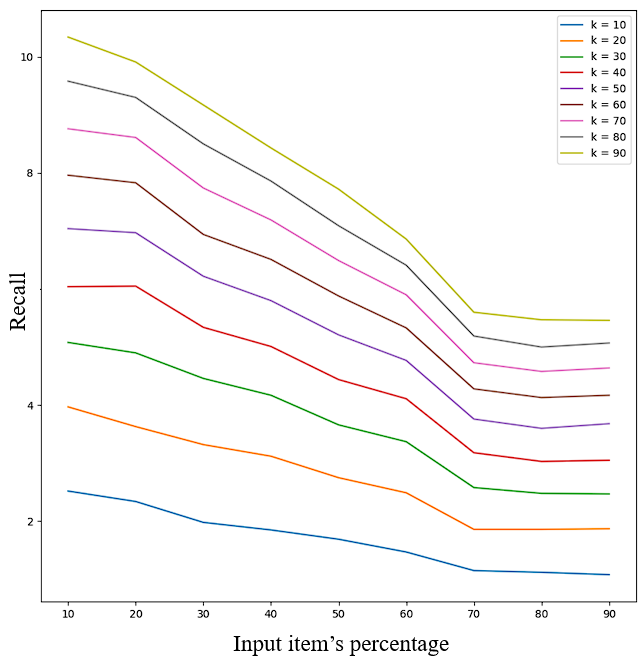
\includegraphics[width=0.7\linewidth]{content/resources/images/fashion-recommendation/chapter4-masked-ratio.png}
    \caption{Recall score on test set with different \textit{Input} item's percentage}
    \label{fig:chapter4-mask-ratio}
\end{figure}

\textbf{Comparison with SOTA methods}

We also compared Outfit Retrieval Transformers (ORT) with other SOTA methods: Type-Aware \cite{Mariya-ECCV18-Learning}, CSA-Net~\cite{Lin-CVPR2020-Fashion}, OutfitTransformer~\cite{Sarkar-CVPRW2022-OutfitTransformer}, and FashionViL~\cite{Han-ECCV2022-FashionViL}, using their published results for the fill-in-the-blank task.

The comparison is performed on outfits of the PolyvoreOutfits test set, where we need to find 1 missing item for each outfit.
The metric recall at rank K is slightly modified by Lin et al.~\cite{Lin-CVPR2020-Fashion} as follows:
\begin{enumerate}
    \item For each missing item, retrieve K items within the same subcategory as that item using KNN (PolyvoreOutfits also contains 153 subcategories with no semantic meaning). If the retrieved K items contain the original item, mark the recommendation correct.
    \item The recall score equals the number of correct recommendations divided by the total number of missing items and multiplied by 100.
\end{enumerate} 

The comparison result is shown in \autoref{table:chapter4-outfit-sota-compare}, showing that our model cannot achieve as high results as other methods in the fill-in-the-blank problem. 

\begin{table}[ht!]
\centering
\begin{tabular}{l l c c c}
\hline
 Method & Published                                & R@10        & R@30         & R@50         \\ \hline
Type-Aware~\cite{Mariya-ECCV18-Learning} & ECCV 2018         & 3.66          & 8.26           & 11.98          \\
CSA-Net~\cite{Lin-CVPR2020-Fashion} & CVPR 2020            & 5.93          & 12.31          & \textbf{17.85} \\
OutfitTransformer~\cite{Sarkar-CVPRW2022-OutfitTransformer}  & CVPRW 2022 & \textbf{6.53} & 12.12          & 16.64          \\ 
FashionVIL~\cite{Han-ECCV2022-FashionViL} & ECCV 2022        & 5.83          & \textbf{12.61} & 17.49          \\ \hline
\textbf{ORT}   & \textbf{Ours}                          & 4.19          & 8.55           & 11.96          \\ \hline
\end{tabular}
\caption{Recall at rank K (R@K) score between our method and other SOTA}
\label{table:chapter4-outfit-sota-compare}
\end{table}

\autoref{fig:chapter4-irt-samples} shows some false recommendation samples. From our perspective, the recommendation results are still acceptable. Indeed, fashion taste varies among individuals, and a reasonable recommendation for one person may not be the same for another. 

\begin{figure}[h!]
    \centering
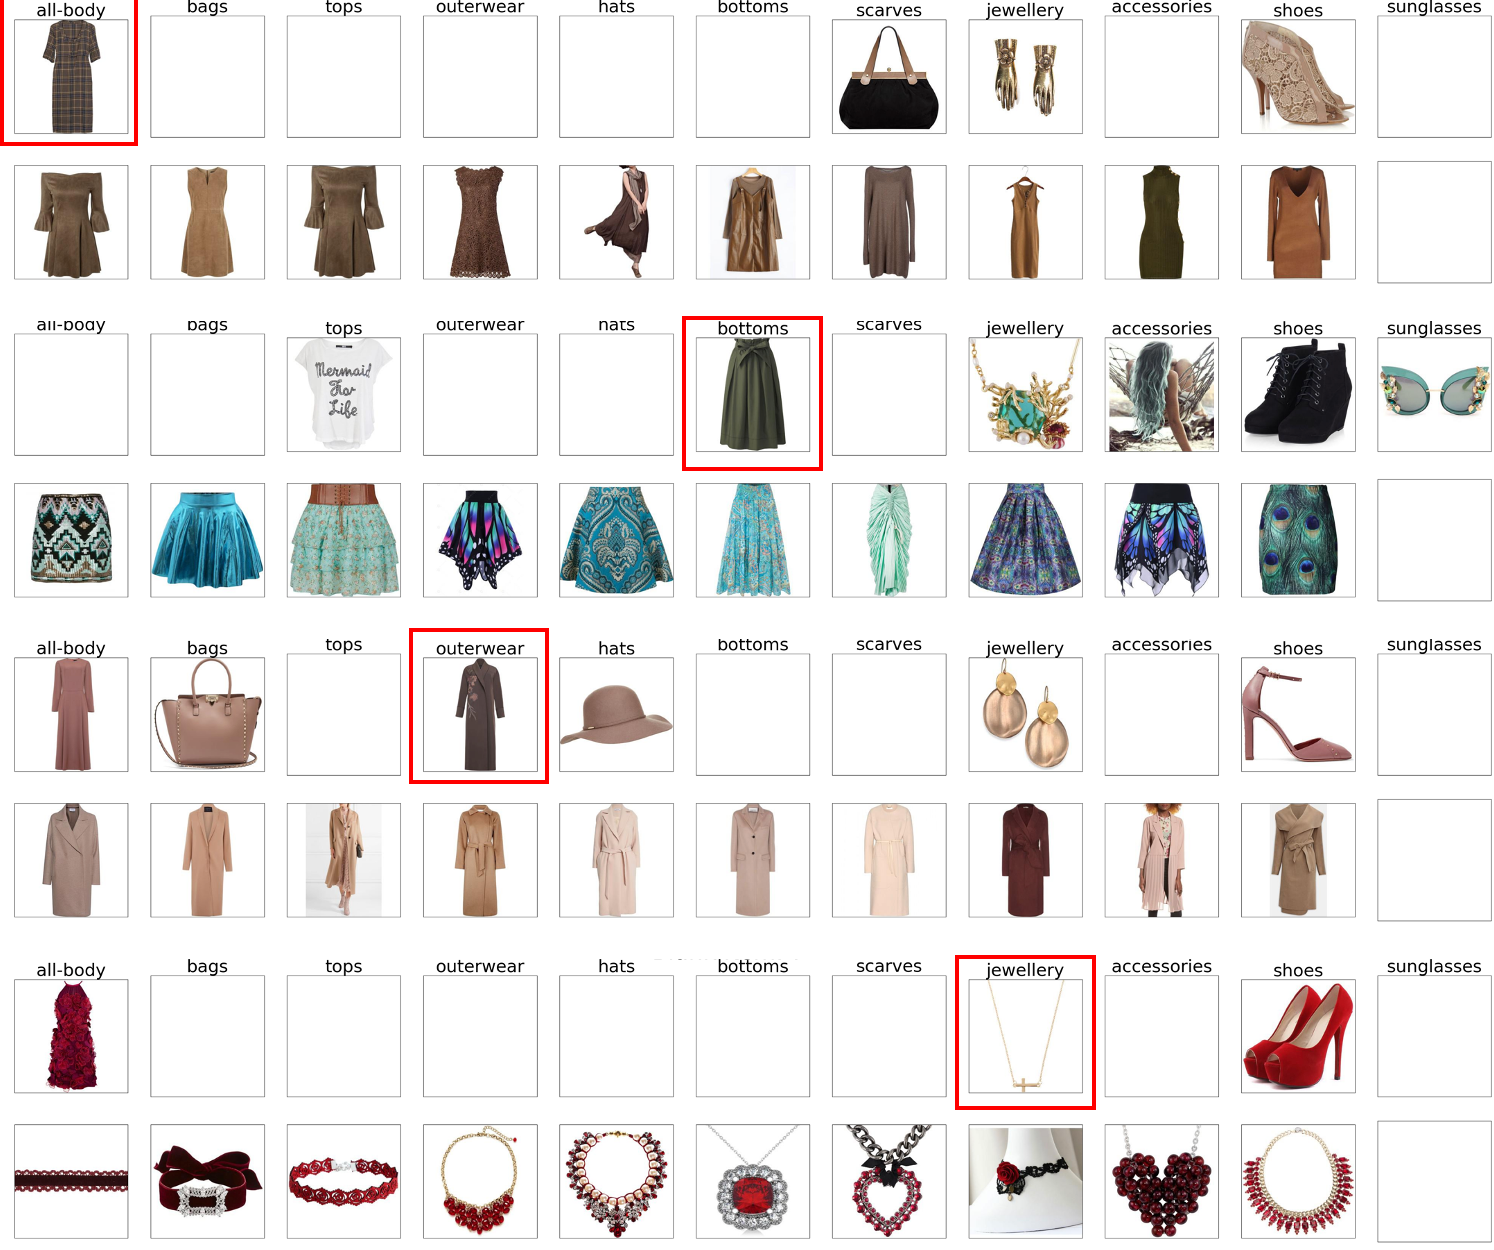
\includegraphics[width=\linewidth]{content/resources/images/fashion-recommendation/chapter4-ort-samples.png}
    \caption{False recommendation according to the ground-truth missing items (marked as red). The following line shows the top 10 items recommended by Outfit Retrieval Transforms.}
    \label{fig:chapter4-irt-samples}
\end{figure}

\subsection{Text feedback-guided item retrieval evaluation}
According to Baldrati's published work~\cite{Baldrati-CVPR2022-Conditioned}, their fine-tuned CLIP and Combiner models are evaluated on the FashionIQ validation set. 
\autoref{fig:fashioniq-val} shows the number of items of each category in the FashionIQ validation set.

\begin{figure}[ht!]
    \centering
    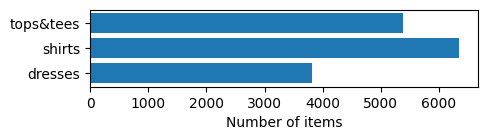
\includegraphics[width=0.7\linewidth]{content/resources/images/fashion-recommendation/chapter4-fashioniq-val.png}
    \caption{The number of items of each category in FashionIQ validation set}
    \label{fig:fashioniq-val}
\end{figure}

The FashionIQ validation set also contains 12,034 triplet pairs. Each triplet pair comprises a reference image, relative feedback, and a target image.
This format allows for the calculation of the recall at rank K metric, which can be computed as follows:
\begin{enumerate}
    \item For each triplet, retrieve K items within the same category as the reference image using KNN. If the retrieved K items contain the target item, mark the recommendation correct.
    \item The recall score equals the number of correct recommendations divided by the total number of triplet pairs and multiplied by 100.
\end{enumerate} 
The evaluation results are shown in \autoref{table:clip4cir}.

\begin{table*}[htb!]
    \centering
    \setlength\tabcolsep{0pt}
    \begin{tabular*}{\linewidth}{@{\extracolsep{\fill}} c ccc ccc ccc ccc}
        \hline 
    \multirow{2}{*}{Method} & \multicolumn{2}{c}{Shirt} & & \multicolumn{2}{c}{Dress} & & \multicolumn{2}{c}{Toptee} & & \multicolumn{2}{c}{Average} \\
    
    \cline{2-3} \cline{5-6} \cline{8-9} \cline{11-12}
&R@10	&R@50 & &R@10	&R@50 & &R@10	&R@50 & &R@10	&R@50 & \\
\hline
CLIP4Cir\cite{Baldrati-CVPR2022-Effective} & 36.36 & 58.00 & & 31.63 & 56.67 & & 38.18 & 62.42 & & 35.39 & 59.03\\
\hline
    \end{tabular*}
    \caption{Recall at rank K (R@K) on the FashionIQ validation set}
    \label{table:clip4cir}
\end{table*}


\subsection{Approximate searching evaluation}

While evaluating an approximate searching method, besides the query time, we also utilized the recall at rank 100 metric with some customization:
\begin{enumerate}
    \item Use K-Nearest Neighbor to query 100 nearest items in the dataset.
    \item Use the approximate method to query 100 nearest items in the dataset.
    \item The metric result is the number of items that belong to both query results.
\end{enumerate}

As we are going to recommend items from the PolyvoreOutfits dataset~\cite{Mariya-ECCV18-Learning} in our application, we used that dataset to compare the effectiveness of searching methods. We additionally appended it with 523,392 items from the DeepFashion dataset~\cite{Liu-CVPR2016-DeepFashion} to investigate the time complexity of approximate searching methods. As a result, there were over 774,400 items in total to index.
Because all approximate searching methods contain multiple parameters to fine-tune, we conducted multiple experiments on the merged dataset to find the appropriate trade-off parameters for each method:
\begin{itemize}
    \item IVF: we chose $nlist$ from the list $\{32, 64, 128, 256, 512,$ $ 1024, 4096, 16384\}$. With each $nlist$ value, we increased the $nprobe$ value until it achieved the average recall of 98.
    \item ANNOY: we chose $n\_tree$ from the list $\{32, 64, 128, 256, 512\}$. With each $n_tree$ value,  we increased the $search\_k$ value until it achieved the average recall of 98.
    \item HNSW: we chose $M$ from the list $\{4, 16, 32, 64, 128\}$, $efConstruction$ from the list $\{8, 16, 32, 64\}$ and ${efSearch}$ from the list $\{32, 64, 128, 256\}$. Subsequently, we removed all setups not achieving the average recall of 98. 
\end{itemize}
We picked the setup having the fastest average query time for each method and compared those methods with KNN on both the merged dataset and PolyvoreOutfits dataset in terms of query time, recall score and memory usage.

\autoref{table:chapter4-ivf} and \autoref{table:chapter4-annoy} show various settings for Inverted File Index (IVF) and Approximate Nearest Neighbor Oh Yeah (ANNOY) that achieve the minimum average recall score of 98. 

As for Hierarchical Navigable Small Worlds (HNSW), \autoref{fig:chapter4-hnsw-full} illustrates the recall score of all settings we prepared. The experiment results were just as we expected; higher values of $M$, $efConstruction$, and $efSearch$ led to higher recalls. \autoref{table:chapter4-hnsw-lite} shows the results after inserting the query time and removing all settings, not achieving 0.98 recall. 

\begin{table}[h!]
\centering
\begin{tabular}{c c c c}
\hline
\textit{nlist} & \textit{nprobe} & Query time (ms)  & Recall         \\ \hline
32 & 8 & 73 & 99.55 \\
64 & 8 & 37.44 & 98.26 \\
128 & 16 & 38.65 & 99.39 \\
256 & 16 & 18.72 & 98.23 \\
512 & 24 & 14.78 & 98.28 \\
1024 & 40 & 12.77 & 98.41 \\
\textbf{4096} & \textbf{88} & \textbf{8.05} & \textbf{98.11} \\
16384 & 176 & 10.14 & 98.08
\\ \hline
\end{tabular}
\caption{Some settings for IVF achieving average recall score of 98}
\label{table:chapter4-ivf}
\end{table}

\begin{table}[h!]
\centering
\begin{tabular}{c c c c}
\hline
\textit{n\_tree} & \textit{search\_k} & Query time (ms)  & Recall         \\ \hline
32 & 53248 & 15.16 & 98.10 \\
64 & 45056 & 12.92 & 98.01 \\
\textbf{128} & \textbf{49152} & \textbf{12.66} & \textbf{98.07} \\
256 & 49512 & 17.39 & 98.10 \\
512 & 49512 & 13.79 & 98.01 
\\ \hline
\end{tabular}
\caption{Some settings for ANNOY achieving average recall score of 98}
\label{table:chapter4-annoy}
\vspace{1cm}
\end{table}

\begin{figure}[h!]
    \centering
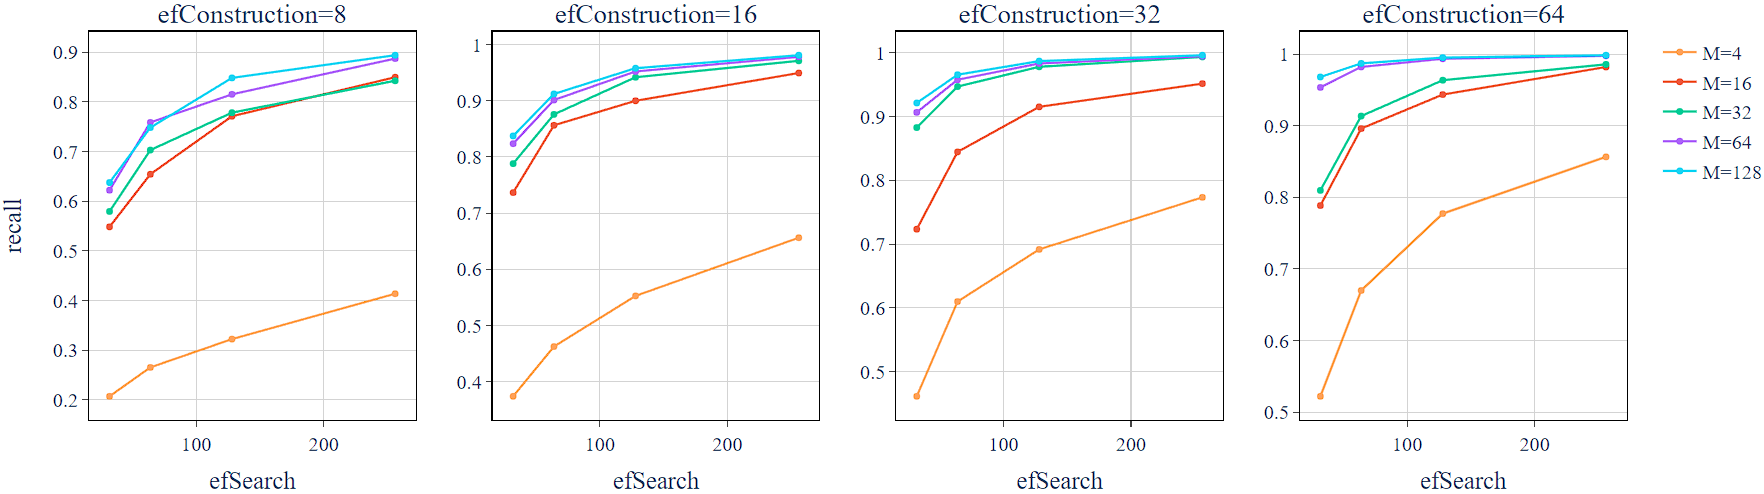
\includegraphics[width=\linewidth]{content/resources/images/fashion-recommendation/chapter4-hnsw-full.png}
    \caption{Recall score for multiple HNSW setups}
    \label{fig:chapter4-hnsw-full}
\end{figure}

\begin{table}[h!]
\centering
\begin{tabular}{c c c c c}
\hline
\textit{M} & \textit{efConstruction} & \textit{efSearch} & Query time (ms)  & Recall         \\ \hline
64 & 64 & 64   & 2.42 & 98.21 \\
128 & 64 & 64  & 5.37 & 98.71 \\
\textbf{32} & \textbf{32} & \textbf{128}  & \textbf{1.72} & \textbf{98.01} \\
64 & 32 & 128  & 3.05 & 98.33 \\
128 & 32 & 128 & 3.85 & 98.71 \\
64 & 64 & 128  & 4.85 & 99.35 \\
128 & 64 & 128 & 3.92 & 99.52 \\
128 & 16 & 256 & 3.91 & 98.09 \\
32 & 32 & 256  & 3.66 & 99.36 \\
64 & 32 & 256  & 5.26 & 99.48 \\
128 & 32 & 256 & 4.19 & 99.63 \\
16 & 64 & 256  & 2.75 & 98.20 \\
32 & 64 & 256  & 3.92 & 98.57 \\
64 & 64 & 256  & 6.99 & 99.76 \\
128 & 64 & 256 & 7.27 & 99.85
\\ \hline
\end{tabular}
\caption{Some settings for HNSW achieving average recall score of 98}
\label{table:chapter4-hnsw-lite}
\end{table}

From the comparison in \autoref{table:chapter4-ivf}, \autoref{table:chapter4-annoy}, and \autoref{table:chapter4-hnsw-lite}, we decided to use $nlist = 4096$ and $nprobe = 88$ for IVF; $n\_tree = 128$ and $search\_k = 49152$ for ANNOY; and $M = 32$, $efConstruction = 32$, and $efSearch = 128$ for HNSW. 

\begin{figure}[h!]
    \centering
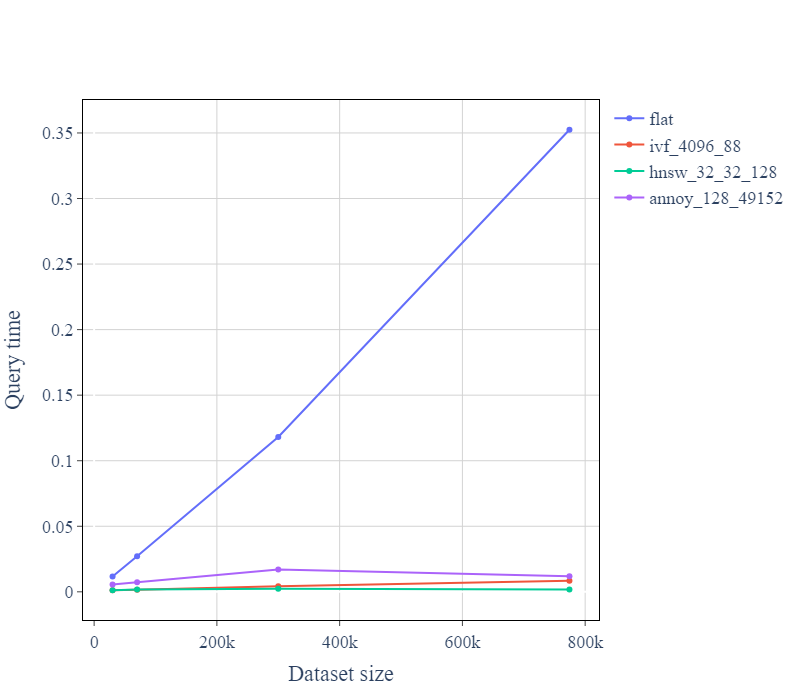
\includegraphics[width=\linewidth]{content/resources/images/fashion-recommendation/chapter4-time-complex.png}
    \caption{Query time of nearest neighbor methods}
    \label{fig:chapter4-time-complex}
\end{figure}

Using these settings, we evaluated the time complexity between KNN, IVF, ANNOY, and HNSW. We subsequently selected 30.000, 70.000, 300.000, and all items from the merged dataset (PolyvoreOutfits~\cite{Mariya-ECCV18-Learning} and DeepFashion~\cite{Liu-CVPR2016-DeepFashion}) to run those algorithms. \autoref{fig:chapter4-time-complex} illustrates the result, showing that all investigated approximate methods run significantly faster than KNN and have nearly constant runtime. This experiment has proven the scalability of approximate searching methods. 

Additionally, we evaluated the query time, recall score and memory usage of these approximate methods on the PolyvoreOutfits dataset and compared them with those of KNN (\autoref{table:chapter4-ann-all}). In summary, HNSW outperforms all other methods regarding query time while using nearly the same memory as KNN and maintaining a recall score of 0.98.



\begin{table}[h!]
\centering
\begin{tabular}{c c c c c}
\hline
Method & Query time (ms) & Recall & Memory (GB) \\ \hline
KNN & 35.24 & 100  & 0.76 \\
IVF & 8.39 & 98.45 & 0.78 \\
ANNOY & 11.83 & 98.39 & 1.2 \\
\textbf{HNSW} & \textbf{1.80} & \textbf{98.11} & \textbf{0.84}
\\ \hline
\end{tabular}
\caption{Performance of searching methods on PolyvoreOutfits}
\label{table:chapter4-ann-all}
\end{table}
